\begin{multicols}{2}
\minpurp{DES:}
m = 64 Bits; 	k = 56 Bits\\
Aus k werden 16 Rundenschlüssel $k_i$ mit 48 Bit generiert;

\minisec{Verschlüsseln:}
Führe Anfangspermutation durch;\\
Ablauf einer Runde i:
\begin{enumerate}
\item Halbiere die nachricht m in x und y: $m \to (x,y)$
\item  Aus (x,y)berechne $(x \oplus f(k_i,y),y)$

 mit $f(k_i,x) = P(S(E(x)\oplus k_i))$\\
	S= Substitution (ersetzten des Blocks)\\
	P= Permutation (Umsortieren der Bits)
\end{enumerate}

\minisec{Entschlüsseln:}
Führe Verschlüsseln in Umgekehrter Reihenfolge durch

\minpurp{AES:}
m= 128 Bits;	k= 128, 192 oder 256 Bits		\\
Rundenanzahl ($N_r$): Für k= 128: 10 k= 192: 12 k= 256: 14

Zustandsmatrix:  4x4 Matrix

\minisec{Ablauf:}
\begin{enumerate}
\item initialisiere Zustandsmatrix mit m
\item bilde $Zustandsmatrix \oplus k_0$
\item for i = 1 bis i= $N_R-1$
\begin{enumerate}
\item 	S-Box:
\item	ZeilenShift(1. um 0, 2. um 1 ...)
\item 	MixColumns
\item 	bilde $Zustandsmatrix \oplus k_0$
\end{enumerate}
\item S-Box
\item Verschiebe die Zeilen der Matrix
\item MixColumns
\end{enumerate}\end{multicols}%
%
\minpurp{Modes of Operation: (r=Blocklänge)}		
\begin{itemize}%
\item ECB: Electronic Codebook Mode \\
			$c_i = E(m_i)$		( Blöcke einzeln Verschlüsseln)\\
			Fehler: nur betroffener Block
\item CBC: Cipher-Block Chaining Mode	\\
			Wähle zufälliges Kryptogramm $c_0$		(Startwert, wird mitgeschickt)\\
			$c_i = E(m_i \oplus c_{i-1})$			(Verschlüssle Nachricht $\oplus$ voriges Kryptogramm\\
			Fehler: betroffener Block, Bitfehler im folgenden
\item CFB: Cipher Feedback Mode: \\
			$c_i = m_i \oplus msb_r(E(x_i))$	(nimm die vordersten r Bits aus $E(x)$ und XORe)\\
			$x_{x_i+1} = lsb_{|x|-r}(x_i) || c_i$      (shifte $c_i$ in x ein)\\
			Fehler: Fehler in den folgenden $\dfrac{\text{Länge von m (DES/AES)}}{\text{\textbf{r}}}$ Blöcken; \\
			zus. bei Bitfehlern => Bitfehler an gleicher Stelle
\item OFB: Output Feedback Mode:\\
			$c_i = m_i \oplus msb_r(E(x_i))$ 	(siehe CFB)\\
			$x_{i+1} = E(x_i)		$		(x als Pseudozufallsgenerator)\\
			Fehler: verloren = alle Folgenden, Bitfehler = Bitfehler an gleicher Stelle
\end{itemize}




\newcommand{\Generate}{(x^8 + x^4 + x^3 +x +1)}

\minisec{S-Box AES}
In jedem Feld der Zustandsmatrix
\begin{enumerate}
\item $x \rightarrow x^-1 mod \Generate $ (\Euklid im \textcolor{purple}{Polynomring})
\item $x \rightarrow Ax +b$ mit \\ 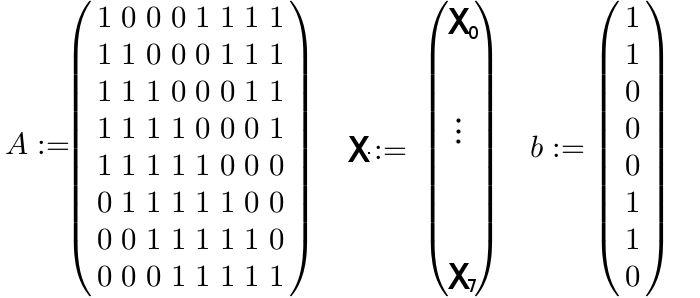
\includegraphics[width=23em]{AES}
\end{enumerate}

\newcommand{\ao}{\textcolor{red}{a0}}
\newcommand{\ai}{\textcolor{blue}{a1}}
\newcommand{\aii}{\textcolor{green}{a2}}
\newcommand{\aiii}{\textcolor{olive}{a3}}

\minisec{Mixcolumns}
(Hinweis: alle Koeffizienten sind mod $\Generate$\\
Betrachte Spalte $a=(\ao,\ai,\aii,\aiii)$ als Polynom \\
\rule{0.5cm}{0pt} $a(X)= \aiii \cdot X^3 + \aii \cdot X^2 + \ai \cdot X^1 + \ao$\\
$a(X) \rightarrow a(X) \cdot ( 03 \cdot X^3 + 01 \cdot X^2 + 01 \cdot X^1 + 02) mod (X^4 +1)$